% This file was created with tikzplotlib v0.10.1.
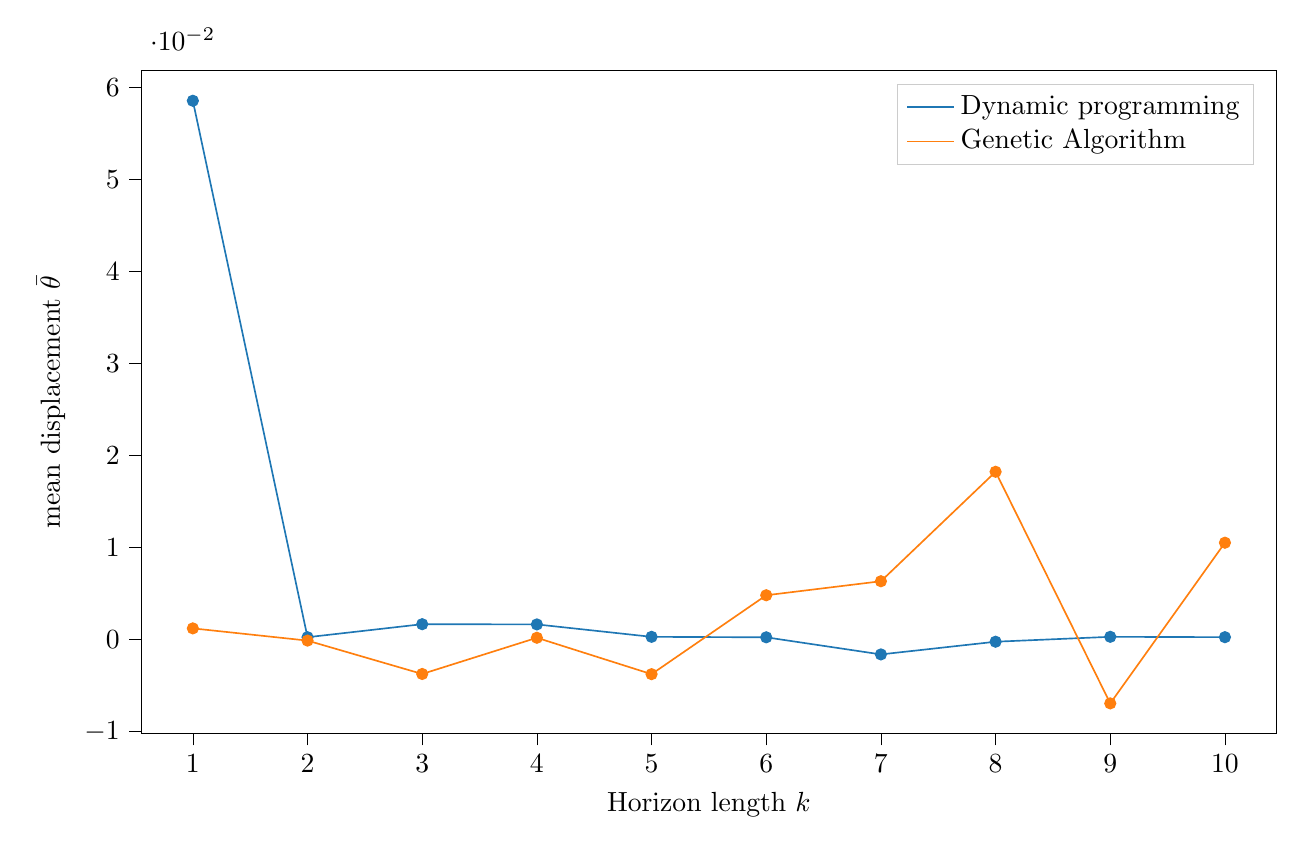
\begin{tikzpicture}

\definecolor{darkgray176}{RGB}{176,176,176}
\definecolor{darkorange25512714}{RGB}{255,127,14}
\definecolor{lightgray204}{RGB}{204,204,204}
\definecolor{steelblue31119180}{RGB}{31,119,180}

\begin{axis}[
height=10cm,
legend cell align={left},
legend style={fill opacity=0.8, draw opacity=1, text opacity=1, draw=lightgray204},
tick align=outside,
tick pos=left,
width=16cm,
x grid style={darkgray176},
xlabel={Horizon length \(\displaystyle k\)},
xmin=0.55, xmax=10.45,
xtick style={color=black},
y grid style={darkgray176},
ylabel={mean displacement \(\displaystyle \bar{\theta}\)},
ymin=-0.0102294246041926, ymax=0.0618486485862511,
ytick style={color=black}
]
\addplot [draw=steelblue31119180, fill=steelblue31119180, forget plot, mark=*, only marks]
table{%
x  y
1 0.05857237253214
2 0.000241663487924673
3 0.0016577343827794
4 0.00163299242418985
5 0.000283728116017774
6 0.000230738630696369
7 -0.0016280707170349
8 -0.000248366194677426
9 0.0002859815510046
10 0.000245708105717786
};
\addplot [draw=darkorange25512714, fill=darkorange25512714, forget plot, mark=*, only marks]
table{%
x  y
1 0.00120287093401887
2 -0.000127070926711933
3 -0.00375526347681442
4 0.000182076932587297
5 -0.00377604893428223
6 0.00480465386304015
7 0.00632811648038798
8 0.018230514409664
9 -0.00695314855008153
10 0.0105170875079598
};
\addplot [semithick, steelblue31119180]
table {%
1 0.05857237253214
2 0.000241663487924673
3 0.0016577343827794
4 0.00163299242418985
5 0.000283728116017774
6 0.000230738630696369
7 -0.0016280707170349
8 -0.000248366194677426
9 0.0002859815510046
10 0.000245708105717786
};
\addlegendentry{Dynamic programming}
\addplot [semithick, darkorange25512714]
table {%
1 0.00120287093401887
2 -0.000127070926711933
3 -0.00375526347681442
4 0.000182076932587297
5 -0.00377604893428223
6 0.00480465386304015
7 0.00632811648038798
8 0.018230514409664
9 -0.00695314855008153
10 0.0105170875079598
};
\addlegendentry{Genetic Algorithm}
\end{axis}

\end{tikzpicture}
